\documentclass[A4,12PT, english, twocolumn]{journal}
\usepackage{amsmath,amssymb,amsfonts}
\usepackage[margin=0.7in]{geometry}
\usepackage{graphicx}
\usepackage{enumitem}
\usepackage{xcolor}
\usepackage{hyperref}
\usepackage{tabularray}
\usepackage{multicol}
\usepackage{tikz}
\usepackage{circuitikz}
\usepackage{scalerel}
\usepackage{pict2e}
\usepackage{tkz-euclide}
\usetikzlibrary{calc}
\usetikzlibrary{patterns,arrows.meta}
\usetikzlibrary{shadows}
\usetikzlibrary{external}

%pgfplots
\usepackage{pgfplots}
\pgfplotsset{compat=newest}
\usepgfplotslibrary{statistics}
\usepgfplotslibrary{fillbetween}

\def\infinity{\rotatebox{90}{8}}

% Hiperlink
\hypersetup{
    colorlinks=true,
    linkcolor=blue,
    filecolor=magenta,      
    urlcolor=cyan,
    pdftitle={Overleaf Example},
    pdfpagemode=FullScreen,
}
%\usepackage{style}
\NewDocumentCommand{\Log}{o}{%
\IfNoValueTF{#1}{}{{}^{#1}\!}\log}%
  
%command buat logaritma dengan basisnya di pojok kiri
%\textheight=17cm
%\textwidth=10cm
%\usepackage{blindtext}
\setenumerate[1]{itemsep=0,5cm}
\setenumerate[2]{topsep=5pt, itemsep=5pt, label=\textbf{\Alph*}.}

\title{Matematika Saintek \& Fisika UTUL UGM 2013 Kode 261}
\author{Fauzan Akbar Sukandar Putra \\ \LaTeX}

\begin{document}

\maketitle

%\begin{minipage}{0.5\textwidth}
\begin{enumerate}


%1%
\item Titik pusat lingkaran yang menyinggung garis $y=2$ di $(3,2)$ dan menyinggung garis $y=-x\sqrt3+2$ adalah\dots
    \begin{enumerate}
        \item $(3,\sqrt3)$
        \item $(3,3\sqrt3)$
        \item $(3,2+\sqrt3)$
        \item $(3,2+2\sqrt3)$
        \item $(3,2+3\sqrt3)$
    \end{enumerate}

%2%
\item Diberikan koordinat titik $O(0,0)$, $B(-3,\sqrt7)$, dan $A(a,0)$, dengan $a < 0$. Jika pada segitiga $AOB$, $\angle OAB=\alpha$ dan $\angle OBA=\beta$, maka $\cos \frac{1}{2}(\alpha +\beta )=$\dots
    \begin{enumerate}
        \item $\frac{1}{4}$
        \item $\frac{1}{4}\sqrt{2}$
        \item $\frac{1}{4}\sqrt{6}$
        \item $\frac{1}{4}\sqrt{7}$
        \item $\frac{1}{4}\sqrt{14}$
    \end{enumerate}

%3%
\item Diketahui vektor-vektor $\vec{u}=(a,1,-a)$ dan \\ $\vec{v}=(1,a,a)$. Jika ${{\vec{u}}_{1}}$ vektor proyeksi $\vec{u}$ pada $\vec{v}$, ${{\vec{v}}_{1}}$ vektor proyeksi $\vec{v}$ pada $\vec{u}$, dan $\theta$ sudut antara $\vec{u}$ dan $\vec{v}$ dengan $\cos \theta =\frac{1}{3}$, maka luas jajaran genjang yang dibentuk oleh ${{\vec{u}}_{1}}$ dan ${{\vec{v}}_{1}}$ adalah\dots
    \begin{enumerate}
        \item $\frac{2}{9}\sqrt{2}$
        \item $\frac{2}{9}\sqrt{6}$
        \item $\frac{2}{3}\sqrt{2}$
        \item $\frac{2}{3}\sqrt{6}$
        \item $2$
    \end{enumerate}

%4%
\item Panjang rusuk kubus $PQRS.TUVW$ adalah $6 \; cm$. Titik $X$ pada $TW$, $Y$ pada $UV$ dan $Z$ pada $QR$. Jika $|TX|:|XW|=1:2$, $|UY|:|YV|=2:1$, dan $PXYZ$ membentuk bidang datar, maka volume bangun $TUYX,PQZ$ adalah\dots
    \begin{enumerate}
        \item $108 \; cm^3$
        \item $80 \; cm^3$
        \item $72 \; cm^3$
        \item $60 \; cm^3$
        \item $36 \; cm^3$
    \end{enumerate}

%5%
\item Diketahui limas beraturan $T.ABCD$ dengan alas berbentuk persegi dan tinggi limas $2\sqrt{3} \; cm$. Jika $T'$ proyeksi $T$ pada bidang alas dan titik $P$ adalah perpotongan garis berat segitiga $TBC$, maka panjang sisi alas limas agar $T' P$ tegak lurus segitiga $TBC$ adalah\dots
    \begin{enumerate}
        \item $2 \; cm$
        \item $\sqrt{6} \; cm$
        \item $\sqrt{8} \; cm$
        \item $3 \; cm$
        \item $4 \; cm$
    \end{enumerate}

%6%
\item Garis $g$ merupakan garis singgung kurva \\ $y=2x^2-x-1$ dengan gradien $m$. Jika garis $g$ membentuk sudut $45^\circ$ terhadap garis $2x-y+4=0$, dan $0<m<2$, maka persamaan $g$ adalah\dots
    \begin{enumerate}
        \item $3x+9y+11=0$
        \item $3x+9y-11=0$
        \item $-3x+9y+11=0$
        \item $-3x+9y-11=0$
        \item $3x-9y-11=0$
    \end{enumerate}

%7%
\item Nilai $x$ yang memenuhi pertaksamaan \\ $\sqrt{(625)^{x-2}}>\left(\sqrt{(125)^x} \right)\left(\sqrt[3]{(25)^{6x}} \right)$ adalah\dots
    \begin{enumerate}
        \item $x>-\frac{8}{3}$
        \item $x<-\frac{8}{3}$
        \item $x<-\frac{8}{7}$
        \item $x>-\frac{8}{7}$
        \item $x<-\frac{12}{5}$
    \end{enumerate}

%8%
\item Himpunan semua $x$ yang memenuhi $|x-2|-1 \geq x$ adalah\dots
    \begin{enumerate}
        \item $\left\{ x|0 \leq x \leq \frac{7}{2} \right\}$
        \item $\left\{ x|x \geq 0 \right\}$
        \item $\left\{ x|x \leq \frac{1}{2} \right\}$
        \item $\left\{ x|0 \leq x \leq \frac{5}{2} \right\}$
        \item $\left\{ x|-1 \leq x \leq \frac{1}{2} \right\}$
    \end{enumerate}

%9%
\item Suku banyak $P(x)$ dibagi $x^2-x-2$ mempunyai hasil bagi $Q(x)$ dan sisa $x+2$. Jika $Q(x)$ dibagi $x+2$ mumpunyai sisa $3$, maka sisa $P(x)$ dibagi $x^2+3x+2$ adalah\dots
    \begin{enumerate}
        \item $-11x-10$
        \item $-10x-11$
        \item $11x-10$
        \item $10x+11$
        \item $11x+10$
    \end{enumerate}

%10%
\item Jumlah $n$ suku pertama suatu deret aritmatika dinotasikan dengan $S_n$. Jika suku pertama deret tersebut tak nol dan $S_4, \; S_8,$ dan $S_{16}$ membentuk barisan geometri, $\frac{S_8}{S_4}=$\dots
    \begin{enumerate}
        \item $2$
        \item $4$
        \item $6$
        \item $8$
        \item $10$
    \end{enumerate}

%11%
\item $\lim\limits_{x \longrightarrow 0} \dfrac{1-\cos^3{x}}{x \tan {x}}=$\dots
    \begin{enumerate}
        \item $0$
        \item $\frac{1}{2}$
        \item $\frac{3}{4}$
        \item $\frac{3}{2}$
        \item $3$
    \end{enumerate}

%12%
\item Jika kurva $f(x)=ax^3-bx^2+1$ mempunyai titik ekstrem $(1,-5)$ maka kurva tersebut naik pada\dots
    \begin{enumerate}
        \item $\left\{ x| x \leq 0 \right.$ atau $\left. x \geq 2 \right\}$
        \item $\left\{ x| x \leq 0 \right.$ atau $\left. x \geq 1 \right\}$
        \item $\left\{ x| x \leq -2 \right.$ atau $\left. x \geq 0 \right\}$
        \item $\left\{ x| x \leq -\frac{1}{2} \right.$ atau $\left. x \geq 0 \right\}$
        \item $\left\{ x| x \leq -2 \right.$ atau $\left. x \geq 1 \right\}$
    \end{enumerate}

%13%
\item Dari $15$ anak yang terdiri atas laki-laki dan perempuan akan diambil $2$ anak secara bersamaan. Jika banyak kemungkinan terambil laki-laki dan perempuan adalah $26$, maka selisih jumlah laki-laki dan perempuan adalah\dots
    \begin{enumerate}
        \item $13$
        \item $11$
        \item $9$
        \item $5$
        \item $3$
    \end{enumerate}

%14%
\item Diketahui polinomial $f(x)$ habis dibagi $x-1$. Jika $f'(x)$ dibagi $x-1$ bersisa $a^2$ dan $\lim\limits_{x \longrightarrow 1} \dfrac{f(x)}{x-1}=2a-1$, maka $a=$\dots
    \begin{enumerate}
        \item $-2$
        \item $-1$
        \item $0$
        \item $1$
        \item $2$
    \end{enumerate}

%15%
\item Jika sudut lancip $x$ memenuhi
\begin{center}
    $1={}^2\Log{16}+{}^2\Log{(\sin{x})}+{}^2\Log{(\cos{x})}+{}^2\Log{(\cos{2x})}$
\end{center}
maka $x=$\dots
    \begin{enumerate}
        \item $\frac{\pi}{2}$
        \item $\frac{\pi}{4}$
        \item $\frac{\pi}{6}$
        \item $\frac{\pi}{24}$
        \item $\frac{\pi}{36}$
    \end{enumerate}
    
    
%FISIKA %
%16%
\newpage
\item Dua batang $A$ dan $B$ terbuat dari bahan yang sama. Dalam keadaan netral atau bebas, batang $B$ memiliki panjang dua kali panjang batang $A$ dan luas penampang lintang batang $A$ dua kali luas penampang lintang batang $B$. Jika kedua batang ditegangkan dengan gaya yang sama besar, maka batang $A$ bertambah panjang dengan $x$ dan batang $B$ bertambah panjang dengan $y$ yang memenuhi hubungan\dots
    \begin{enumerate}
        \item $y=\frac{x}{4}$
        \item $y=\frac{x}{2}$
        \item $y=x$
        \item $y=2x$
        \item $y=4x$
    \end{enumerate}
  
%17%
\item Sebuah bola dijatuhkan bebas dari ketinggian $6,4 \; m$ di atas lantai. Pada pantulan pertama oleh lantai, bola mencapai ketinggian maksimum $4,8 \; m$ diatas lantai. Berapa ketinggian maksimum yang dicapai bola pada pantulan yang ketiga\dots
    \begin{enumerate}
        \item $4,2 \; m$
        \item $3,6 \; m$
        \item $3,2 \; m$
        \item $2,7 \; m$
        \item $2,4 \; m$
    \end{enumerate}
     
%18%
\item Massa $1 \; kg$ bergetar selaras sederhana pada sistem pegas dengan tetapan gaya $k=400 \; N/m$. Jika amplitudo getaran tersebut $5 \; cm$, berapa kecepatan massa tersebut pada saat melewati titik setimbang\dots
    \begin{enumerate}
        \item $8 \; m/s$
        \item $4 \; m/s$
        \item $2 \; m/s$
        \item $1 \; m/s$
        \item $0,5 \; m/s$
    \end{enumerate}
   
%19% 
\item Benda bermassa $m$ mula-mula diam di atas lantai licin. Pada saat $t=0$ benda mulai dikenai gaya konstan horizontal sebesar $F$ newton. Setelah gaya bekerja selama $t$ sekon, kecepatan benda tersebut $v \; m/s$. Dari ketentuan-ketentuan di atas, massa benda dapat dinyatakan sebagai\dots
    \begin{enumerate}
        \item $m=\frac{Ft}{v}$
        \item $m=\frac{Ft}{2v}$
        \item $m=\frac{2F}{vt}$
        \item $m=\frac{Fv}{2t}$
        \item $m=\frac{2t}{Fv}$
    \end{enumerate}

%20%
\item Benda bermassa $M$ berbentuk silinder pejal/massif homogen dengan jari-jari $R$ dililit dengan tali halus (massa tali diabaikan). Ujung tali dimatikan di titik tetap dan benda dibiarkan terjatuh berotasi seperti gambar di bawah. Dengan percepatan gravitasi $g$, besar tegangan tali pada sistem tersebut adalah\dots
\begin{center}
    \begin{tikzpicture}
       %\draw[lightgray] (0,0) grid (5,-5);
        \draw[ultra thick] (2.5,0) -- (2.5,-4.5);
        \fill[pattern = north east lines] (0,0) rectangle (5,0.25);
        \draw[ultra thick, red] (0,0) -- (5,0);        
        \draw[ultra thick, draw={shade}] (3,-4.5) circle (14px);
        \shade [left color=blue, right color=red] (3,-4.5) circle (14px);
    \end{tikzpicture}
\end{center}
    \begin{enumerate}
        \item $Mg$
        \item $\frac{2Mg}{3}$
        \item $\frac{Mg}{2}$
        \item $\frac{Mg}{3}$
        \item $\frac{Mg}{4}$
    \end{enumerate}

%21%
\item Sebuah keping cakram disk memiliki momen inersia $I$ berputar dengan kecepatan sudut mula-mula $\omega$. Kemudian dijatuhkan sebuah keping cakram lain tepat di atasnya, sehingga berputar bersama. Bila kecepatan sudut bersamanya adalah $\frac{\omega}{3}$, maka momen inersia keping cakram disk kedua adalah\dots
    \begin{enumerate}
        \item $I$
        \item $2I$
        \item $3I$
        \item $4I$
        \item $5I$
    \end{enumerate}
    
%22% 
\item Dua buah konduktor $A$ dan $B$ terbuat dari bahan yang sama dengan panjang keduanya juga sama. Konduktor $A$ merupakan kawat padat dengan diameter tampang lintang sebesar $1 \; m$, konduktor $B$ merupakan kawat dengan penampang lintang berlubang dengan diameter dalam $1 \; m$ dan diameter luar $2 \; m$. Besar perbandingan nilai hambatan $\frac{R_A}{R_B}$ adalah\dots
    \begin{enumerate}
        \item $4$
        \item $3$
        \item $2$
        \item $\sqrt{2}$
        \item $1$
    \end{enumerate}
    
%23%
\item Partikel $A$ (muatan $Q_A$) dan partikel $B$ (muatan $Q_B$) keduanya diletakkan pada sumbu $x$, dengan partikel $A$ di $x=a$ dan partikel $B$ di $x=-2a$. Partikel $C$ (muatan $Q_C$) yang diletakkan di $x=0$ tidak mengalami gaya listrik bila $Q_B$ sebesar\dots
    \begin{enumerate}
        \item $4 \; Q_A$
        \item $2 \; Q_A$
        \item $Q_A$
        \item $-2 \; Q_A$
        \item $-4 \; Q_A$
    \end{enumerate}
    
%24%  
\item Dalam rangkaian listrik ini, ggl baterai $B$ sebesar $12$ volt akan diukur dengan voltmeter $V$ yang bertahanan dalam sangat besar. Pembacaan voltmeter $V$ memberikan hasil sebesar $10,5$ volt sehingga besar arus listrik yang melewati baterai $B$ adalah\dots
\begin{center}
    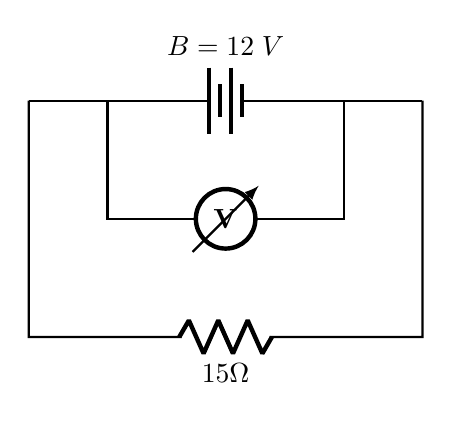
\begin{tikzpicture}
        %\draw[lightgray] (0,0) grid (5,-5);
        \draw[thick] (0,0) to (0,-3) to[R, a=$15\Omega$] (5,-3) to (5,0);
        \draw[thick] (0,0) to[battery, a^={$B=12 \; V$}] (5,0);
        \draw[thick] (1,0) to (1,-1.5) to[voltmeter] (4,-1.5) to (4,0);
    \end{tikzpicture}
\end{center}
	\begin{enumerate}
		\item $0,05 \; A$
		\item $0,1 \; A$
		\item $0,3 \; A$
		\item $0,7 \; A$
		\item $0,9 \; A$
	\end{enumerate}
	
%25%
\item Dua buah kawat listrik yang amat panjang diletakkan dalam posisi sejajar satu sama lain dengan jarak $d$. Arus listrik $I$ dan $2I$ mengalir dalam masing-masing kawat. Lokasi/posisi titik $P$ dari kawat berarus $I$ yang tidak merasakan medan magnet adalah di $x=$\dots
\begin{center}
    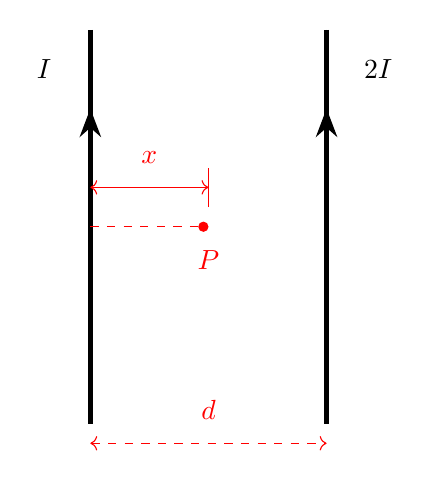
\begin{tikzpicture}
        %GRID
       %\draw[lightgray] (0,0) grid (5,-5);
        %GARIS SEBELAH KIRI
       \draw[ultra thick, -Stealth] (0,-5) -- (0,-1);
       \draw[ultra thick] (0,-2) -- (0,0);
       \draw[ultra thick] (0,0) -- (0,-1) node[midway, left=10pt]{$I$};
        %GARIS SEBELAH KANAN
       \draw[ultra thick, -Stealth] (3,-5) -- (3,-1);
       \draw[ultra thick] (3,0) -- (3,-2);
       \draw (3,0) -- (3,-1) node[midway, right=10pt] {$2I$};
       %GARIS BBAWAH
       \draw[red, dashed, <->] (0,-5.25) -- (3,-5.25) node[midway, above=5pt] {$d$};
       %GARIS P
       \draw[red,dashed,-Circle] (0,-2.5) -- (1.5,-2.5) node[below=5pt]{$P$};
       %GARIS x
       \draw[<->, red] (0,-2) -- (1.5,-2) node[midway, above=5pt] {$x$};
       \draw[red] (1.5,-2.25) -- (1.5,-1.75);
    \end{tikzpicture}
\end{center}
   \begin{enumerate}
        \item $\frac{3}{2}d$
        \item $\frac{4}{3}d$
        \item $d$
        \item $\frac{2}{3}d$
        \item $\frac{1}{3}d$
   \end{enumerate}
   
%26%
\item Sebuah elektron bergerak ke arah sumbu $x$ positif memasuki daerah yang memilik medan listrik sebesar $E$ ke arah sumbu $z$ positif. Agar elektron tadi tetap bergerak lurus dan tidak terbelokkan, maka di daerah tadi ditambahkan dengan medan magnet tertentu berarah pada\dots
    \begin{enumerate}
        \item Sumbu $z$ positif
        \item Sumbu $z$ negatif
        \item Sumbu $x$ positif
        \item Sumbu $x$ negatif
        \item Sumbu $y$ negatif
    \end{enumerate}
  
%27%  
\item Suatu rangkaian listrik $RLC$ seri dihubungkan dengan sumber arus bolak balik dengan tegangan maksimum $100 \; V$. Bila amplitudo tegangan $V_R, \; V_L$ dan $V_C$ ketiganya sama besar satu sama lain, maka $V_R=$\dots
    \begin{enumerate}
        \item $33 \; V$
        \item $50 \; V$
        \item $67 \; V$
        \item $87 \; V$
        \item $100 \; V$
    \end{enumerate}
    
%28%  
\item Gas ideal monoatomik dalam sebuah wadah mengalami kompresi adiobatik. Mula-mula tekanan gas adalah $1$ atmosfer, volumenya $1 \; m^3$ dan suhunya $300 \; K$. Bila setelah ekspansi suhunya menjadi $1200 \; K$, maka volume gas tadi diakhir kompresi adalah\dots
    \begin{enumerate}
        \item $\frac{1}{4} \; m^3$
        \item $\frac{1}{8} \; m^3$
        \item $\frac{1}{16} \; m^3$
        \item $\frac{1}{32} \; m^3$
        \item $\frac{1}{64} \; m^3$
    \end{enumerate}

%29%  
\item Satu mol gas ideal monoatomik dipanaskan pada tekanan konstan $1 \; atm$ sehingga suhu gas tersebut naik dari $0^\circ \; C$ menjadi $100^\circ \; C$. Bila $R$ adalah tetapan gas umum, maka besar perubahan energi dalam (internal) gas adalah\dots
    \begin{enumerate}
        \item $350 \; R$
        \item $250 \; R$
        \item $150 \; R$
        \item $75 \; R$
        \item $50 \; R$
    \end{enumerate}

%30%
\item Sebuah mesin kalor dirancang dapat menyerap kalor pada suhu $527^\circ \; C$ dan membuang kalor tersebut pada suhu $327^\circ \; C$. Dengan adanya input (masukan) kalor sebesar $3000 \; J$ maka besar usaha yang terbesar yang dapat dilakukan oleh mesin yang beroprasi dengan efisiensi maksimum adalah\dots
    \begin{enumerate}
        \item $3000 \; J$
        \item $1600 \; J$
        \item $1200 \; J$
        \item $750 \; J$
        \item $400 \; J$
    \end{enumerate}
 
%31%
\item Sebuah benda berada $20 \; cm$ di sebelah kiri lensa $I$ (panjang fokus $+10 \; cm$). Lensa $II$ (panjang fokus $+12,5 \; cm$) berada $30 \; cm$ di sebelah kanan lensa $I$. Jarak antara benda asli dengan bayangan akhir adalah\dots
    \begin{enumerate}
        \item $\infinity$
        \item $100 \; cm$
        \item $50 \; cm$
        \item $28 \; cm$
        \item $0$
    \end{enumerate}

%32%
\item Cermin datar $R$ berada pada posisi tegak dan diputar mengitari sumbu vertikal $XX'$ dengan kelajuan $100 \; rpm$. Seberkas cahaya mendatar $C$ mengenai cermin $R$. Cahaya terpantul akan terputar dengan kelajuan\dots
\begin{center}
    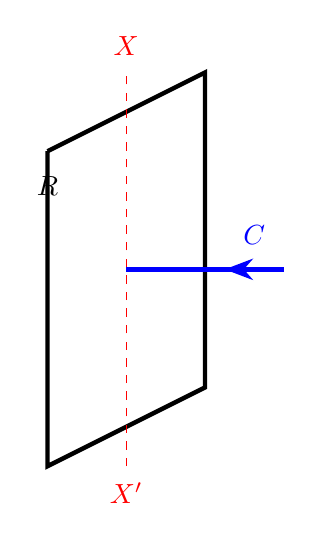
\begin{tikzpicture}
        %GRID
        %\draw[lightgray] (0,0) grid (5,-5);
        %JAJARGENJANG
        \draw[ultra thick] (0,-1) -- (0,-5) -- (2,-4) -- (2,0) -- (0,-1) node[right=10pt, below=5pt] {$R$};
        %GARIS X
        \draw[dashed, red] (1,-5) node[below=2.5pt]{$X'$} -- (1,0) node[above=2.5pt]{$X$};
        %CAHAYA
        \draw[blue, ultra thick] (3,-2.5) -- (1,-2.5);
        \draw[blue, ultra thick, -Stealth] (3,-2.5) -- (2.25,-2.5) node[midway, above=5pt] {$C$};
    \end{tikzpicture}
\end{center}
    \begin{enumerate}
        \item $0 \; rpm$
        \item $100 \; rpm$
        \item $141 \; rpm$
        \item $200 \; rpm$
        \item $10000 \; rpm$
    \end{enumerate}

%33%
\item Umur paruh dari radium adalah $1600$ tahun. Bila sebungkah batu mengandung $0,2$ gram radium, maka jumlah radium dalam batu tersebut $12800$ tahun yang lalu adalah\dots
    \begin{enumerate}
        \item $31,2$ gram
        \item $41,2$ gram
        \item $51,2$ gram
        \item $61,2$ gram
        \item $71,2$ gram
    \end{enumerate}

%34%
\item Jika sebuah atom dimasukkan ke dalam wilayah medan magnet seragam maka sub kulit $d(\ell=2)$ akan pecah menjadi\dots
    \begin{enumerate}
        \item $2$ arah
        \item $4$ arah
        \item $5$ arah
        \item $6$ arah
        \item $7$ arah
    \end{enumerate}

%35%
\item Sebuah asteroid bergerak dalam orbitnya yang berbentuk lingkaran dengan jari-jari $r$ di sekitar matahari. Dengan anggapan bahwa matahari tidak bergerak dan bermassa $M$, sedeng asteroid tersebut bermassa $m$, maka energi mekanik asteroid tersebut adalah\dots
    \begin{enumerate}
        \item $-\frac{GMm}{r}$
        \item $-\frac{GMm}{2r}$
        \item $-\frac{GMm}{2r^2}$
        \item $\frac{GMm}{2r}$
        \item $\frac{GMm}{r}$
    \end{enumerate}

\end{enumerate}
\end{document}  
